% Capítulo 1: fluxograma da média de duas notas com aprovação.
\documentclass[border=4pt]{standalone}
\usepackage[utf8]{inputenc}
\usepackage[T1]{fontenc}
% Estilo comum dos fluxogramas e diagramas de blocos.
\usepackage{tikz}
\usetikzlibrary{arrows.meta, positioning, calc, shapes.geometric, shapes.misc}
\definecolor{navy}{RGB}{23,45,80}
\definecolor{laranja}{RGB}{250,110,29}
\definecolor{cinzalogo}{RGB}{107,114,126}
\definecolor{azul}{RGB}{205,222,247}
\tikzset{
  base/.style={draw=navy, line width=0.9pt, font=\sffamily\small, align=center, inner sep=4pt},
  terminal/.style={base, rounded rectangle, fill=laranja!45, draw=laranja, minimum width=20mm, minimum height=7mm},
  processo/.style={base, rectangle, fill=laranja!12, minimum width=28mm, minimum height=8mm},
  decisao/.style={base, diamond, aspect=2.2, fill=azul, inner sep=1pt, minimum width=30mm},
  es/.style={base, trapezium, trapezium left angle=72, trapezium right angle=108,
             fill=white, minimum width=26mm, minimum height=8mm, trapezium stretches body},
  fluxo/.style={-{Stealth[length=2.2mm]}, navy, line width=0.9pt},
  rotulo/.style={font=\sffamily\small\bfseries, text=navy},
  legenda/.style={font=\sffamily\scriptsize, text=cinzalogo},
  resposta/.style={font=\sffamily\scriptsize\bfseries, text=navy},
}

\begin{document}
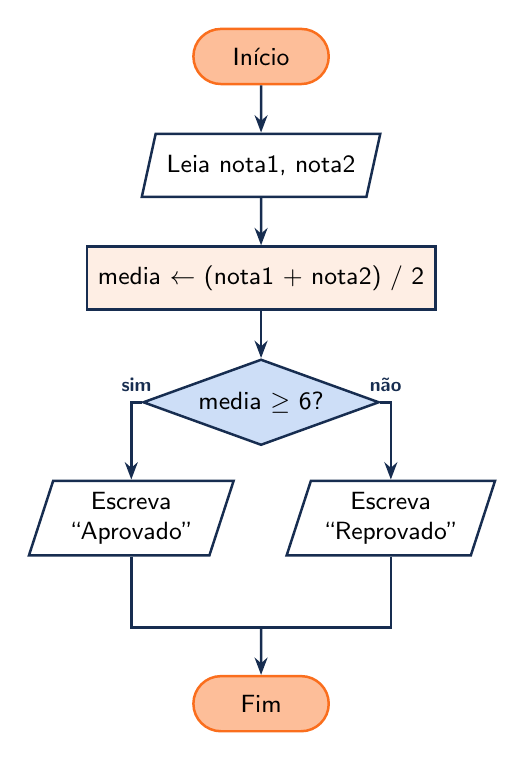
\begin{tikzpicture}[node distance=6mm]
  \node[terminal] (ini) {Início};
  \node[es, below=of ini] (ler) {Leia nota1, nota2};
  \node[processo, below=of ler] (calc) {media $\leftarrow$ (nota1 + nota2) / 2};
  \node[decisao, below=of calc] (dec) {media $\geq$ 6?};
  \node[es, below left=7mm and 4mm of dec] (apr) {Escreva\\``Aprovado''};
  \node[es, below right=7mm and 4mm of dec] (rep) {Escreva\\``Reprovado''};
  \coordinate (junta) at ($(dec.south) + (0, -2.3)$);
  \node[terminal, below=6mm of junta] (fim) {Fim};

  \draw[fluxo] (ini) -- (ler);
  \draw[fluxo] (ler) -- (calc);
  \draw[fluxo] (calc) -- (dec);
  \draw[fluxo] (dec.west) -| node[resposta, pos=0.25, above] {sim} (apr.north);
  \draw[fluxo] (dec.east) -| node[resposta, pos=0.25, above] {não} (rep.north);
  \draw[navy, line width=0.9pt] (apr.south) |- (junta);
  \draw[navy, line width=0.9pt] (rep.south) |- (junta);
  \draw[fluxo] (junta) -- (fim);
\end{tikzpicture}
\end{document}
